\graphicspath{{./Imagenes/an1/}}
\chapter{Cálculo de Resultados para Bolund y Comparación Ciega}
A modo de tener resultados comparables para el ejercicio de comparación ciega organizado por los desarrolladores del experimento de Bolund, se introducen ciertas métricas para la velocidad y para la energía cinética turbulenta \cite{Bechmann2011}.

Para el caso de la velocidad, se adimensionaliza esta de la siguiente forma:
\begin{equation*}
\Delta S_s = \frac{\overline{s} - \overline{s_0}}{\overline{s_0}}
\end{equation*}

Donde $\Delta S_s$ corresponde al \emph{Speedup} simulado, calculado en función de $\overline{s_0}$ que es un valor de referencia para la velocidad ubicado en un punto no perturbado por el terreno (en el experimento de Bolund se utiliza el valor en el mástil M0). Para los resultados presentados en esta tesis los valores de referencia se toman en las coordenadas (55.70313,12.0970) que caen dentro del dominio d08 de simulación.

El valor de $\overline{s_0}$, operativamente, se toma como el promedio temporal entre las 12:00 y 15:00 horas y se calcula para cada nivel vertical del modelo.

Con respecto a la energía cinética turbulenta, esta se adimensionaliza como:
\begin{equation*}
\Delta k_s = \frac{\overline{k}}{\overline{s_0^2}} - \frac{\overline{k_0}}{\overline{s_0^2}}
\end{equation*}
Análogamente al caso anterior, $\overline{k_0}$ es un valor de referencia para la energía cinética turbulenta en el punto del dominio donde hay flujo no perturbado.

De manera referencial, los desarrolladores presentan los siguientes resultados para su comparación ciega de modelos:

\begin{figure}[H]
	\centering
	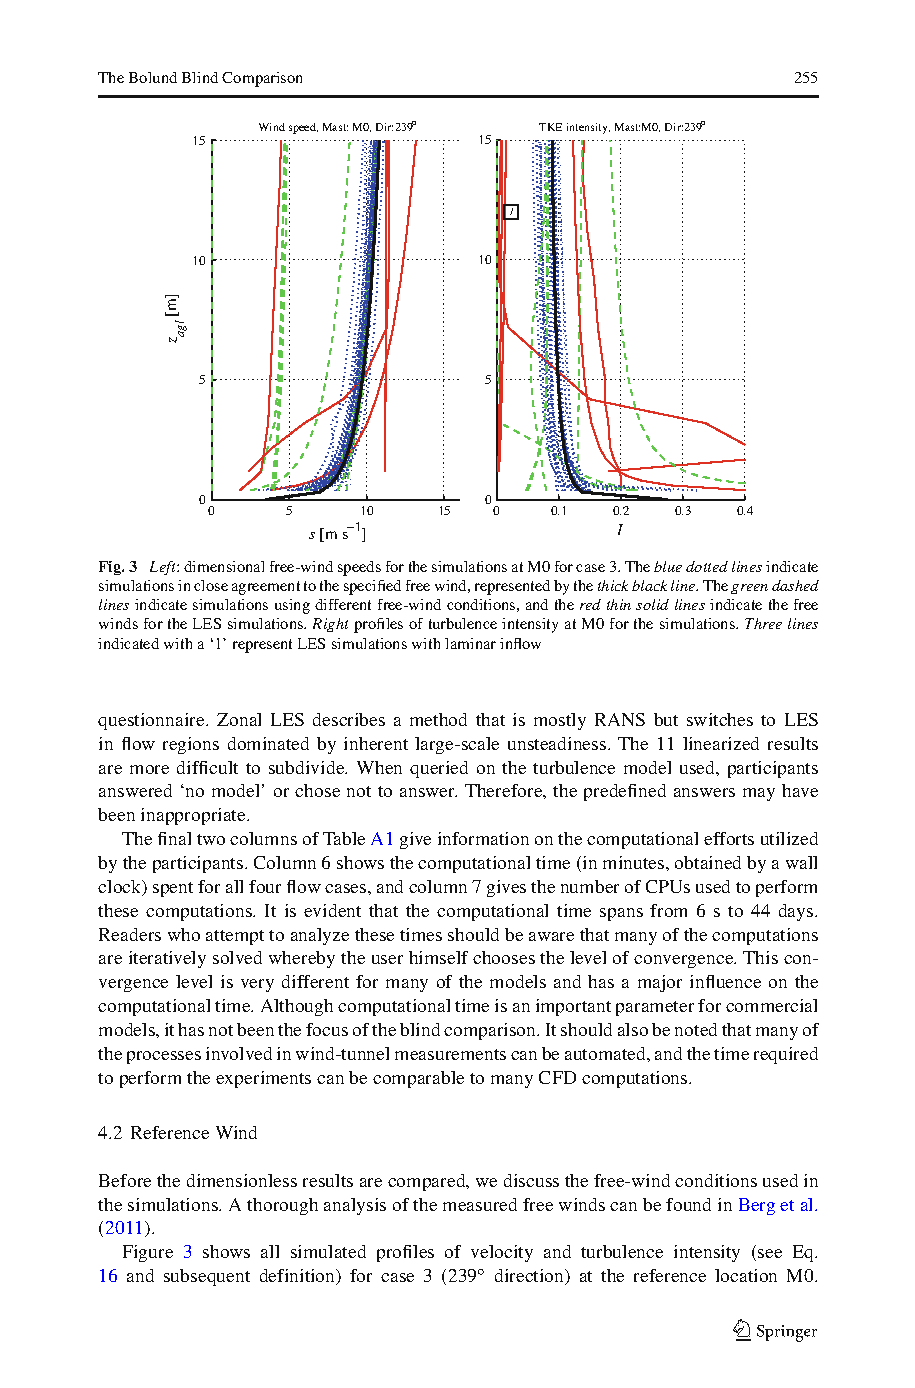
\includegraphics[width=0.85\linewidth,trim={2.7cm 14.3cm 2.0cm 2cm},clip]{bolund1.pdf}%
	\caption{Perfil del viento no perturbado en el punto referencial M0 (ver Figura \ref{fig:05_terreno_bolund}). En línea negra está el perfil entregado por los desarrolladores (para utilizar como condición de borde) y el resto corresponde a distintos modelos. La línea sólida roja corresponde a simulaciones LES.}
	\label{fig:an1_m0}
\end{figure}

\begin{figure}[H]
	\centering
	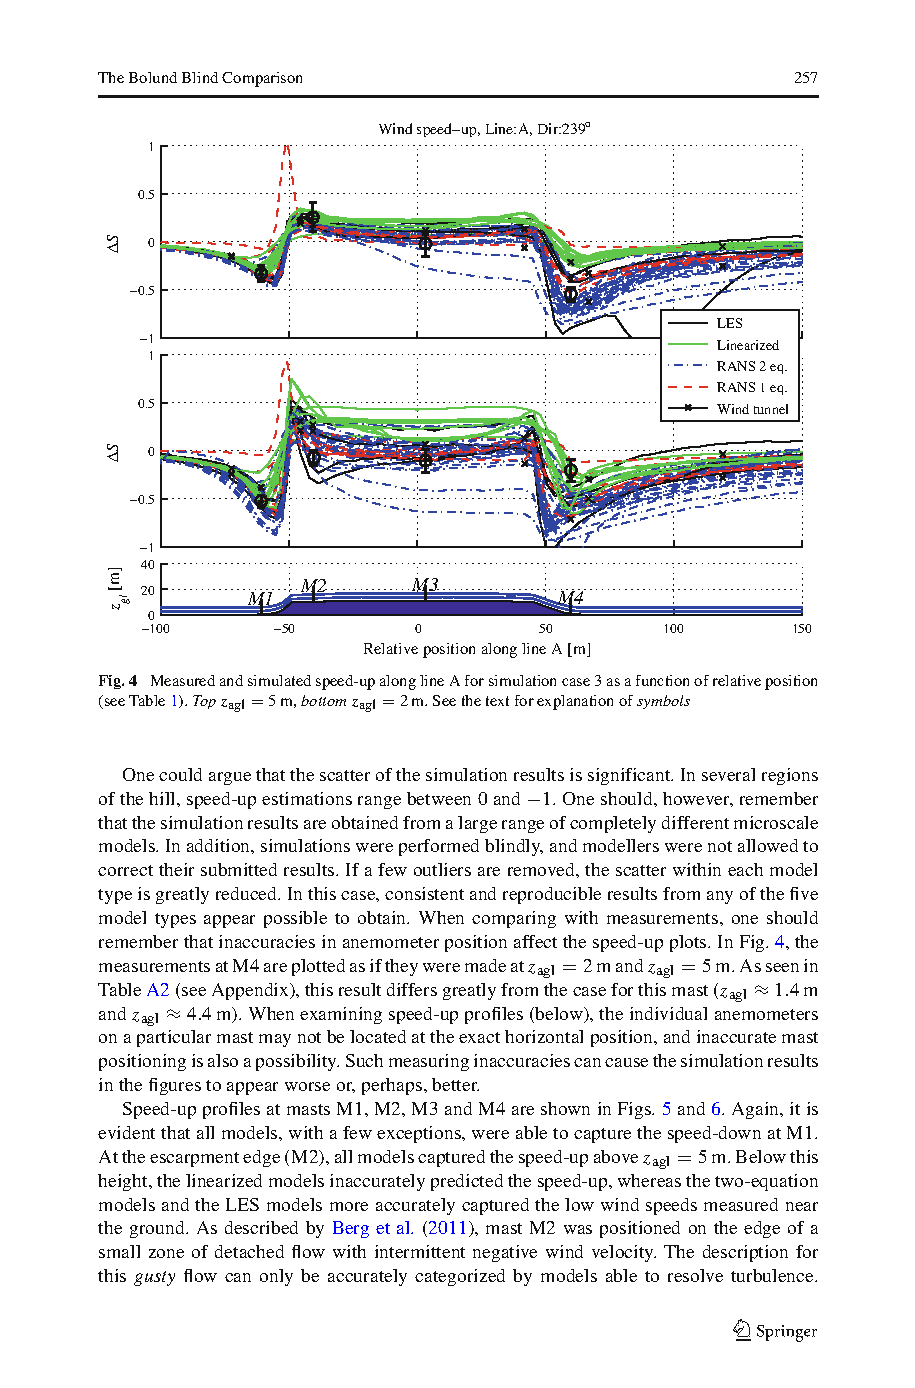
\includegraphics[width=0.9\linewidth,trim={1.7cm 12.3cm 0.9cm 2cm},clip]{bolund2.pdf}%
	\caption{Speedup medido y simulado a través de la sección transversal a $240^\circ$. Arriba: valores para $z=5$ [m]. Abajo: valores para $z=2$ [m].}
	\label{fig:an1_speedup}
\end{figure}

\begin{figure}[H]
	\centering
	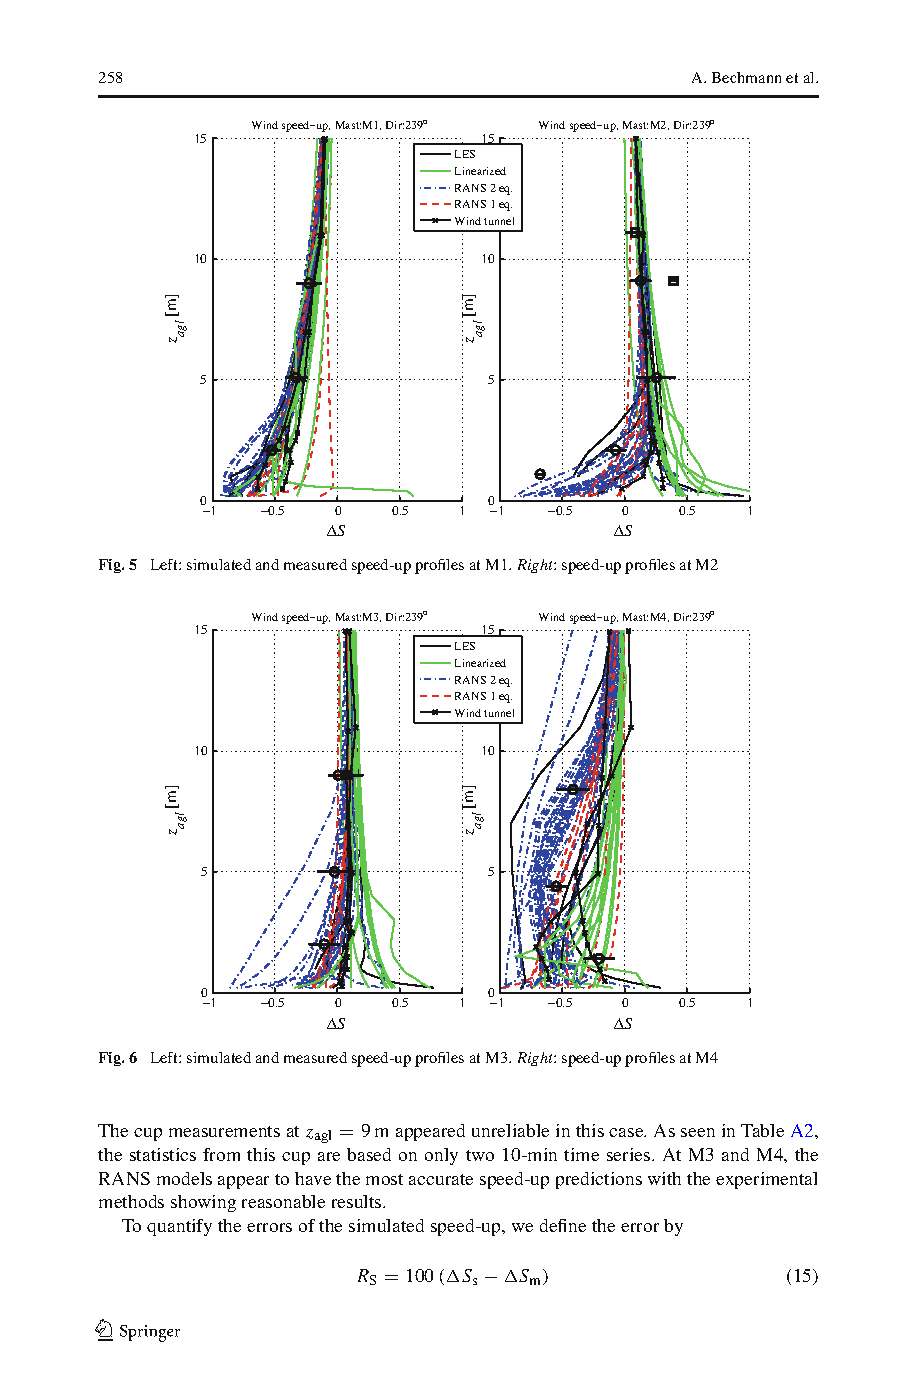
\includegraphics[width=1.0\linewidth,trim={2.7cm 14.4cm 1.9cm 2cm},clip]{bolund3.pdf}%
	
	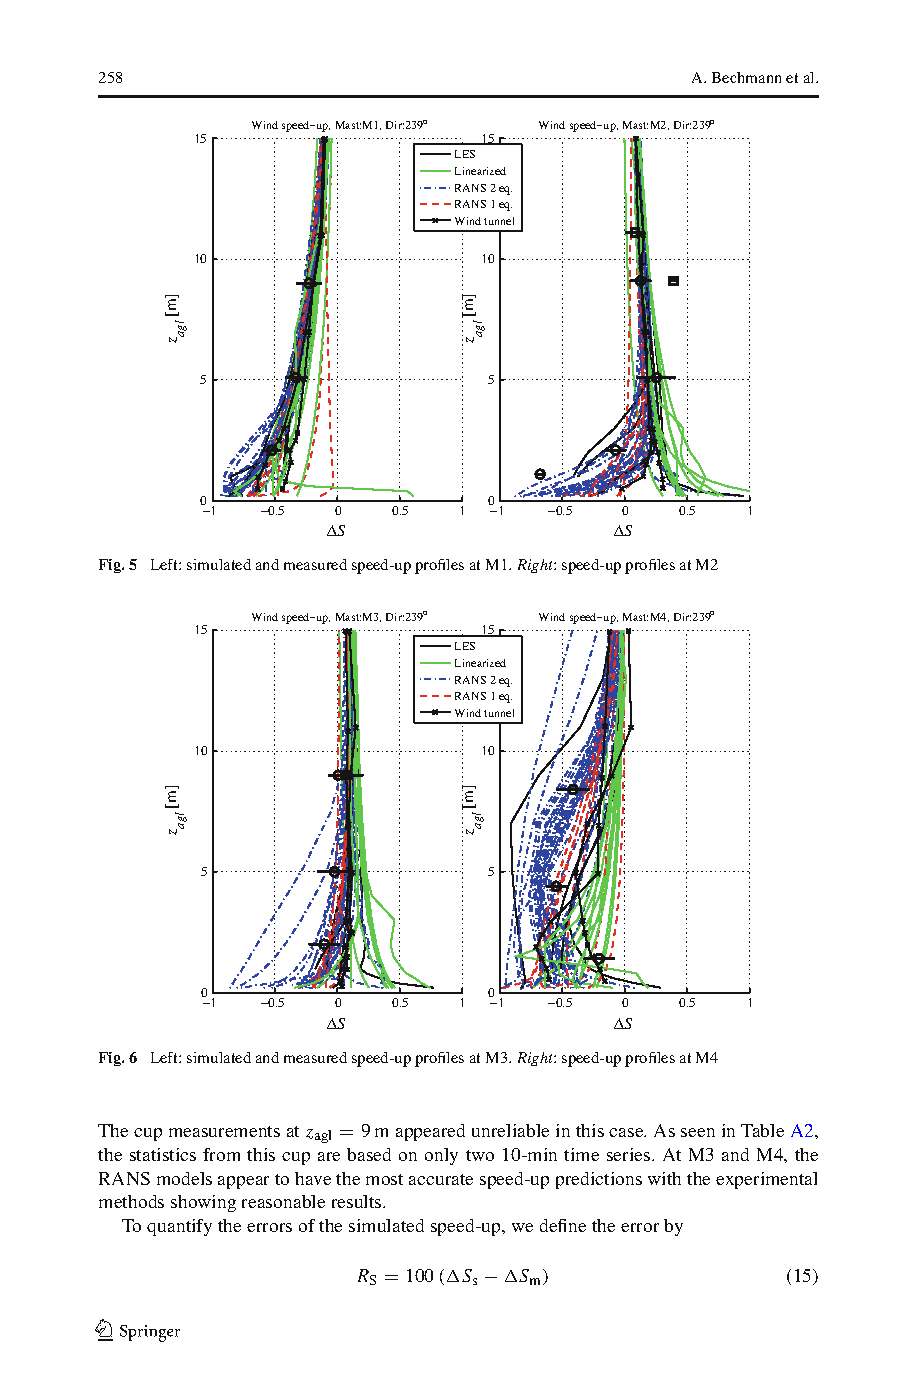
\includegraphics[width=1.0\linewidth,trim={2.7cm 6.0cm 1.9cm 10.3cm},clip]{bolund3.pdf}%
	\caption{Perfil de speedup medido y simulado en los distintos mástiles M1-M4.}
	\label{fig:an1_speed_masts}
\end{figure}

\begin{figure}[H]
	\centering
	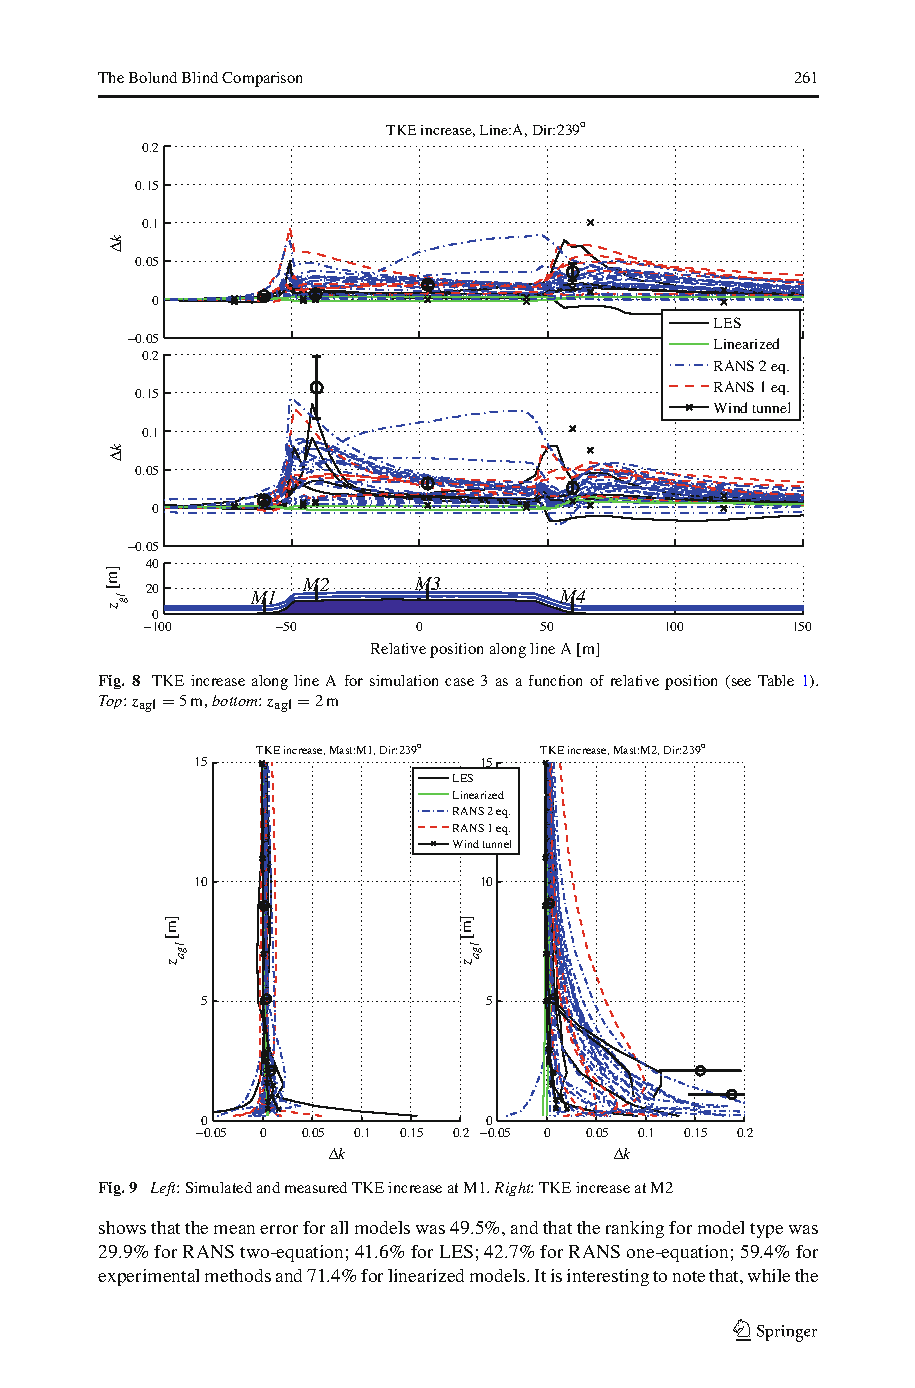
\includegraphics[width=1\linewidth,trim={1.7cm 12.3cm 0.8cm 2cm},clip]{bolund4.pdf}%
	
	\caption{$\Delta k$ medido y simulado a través de la sección transversal a $240^\circ$. Arriba: valores para $z=5$ [m]. Abajo: valores para $z=2$ [m].}
	\label{fig:an1_delta_tke}
\end{figure}

\begin{figure}[H]
	\centering
	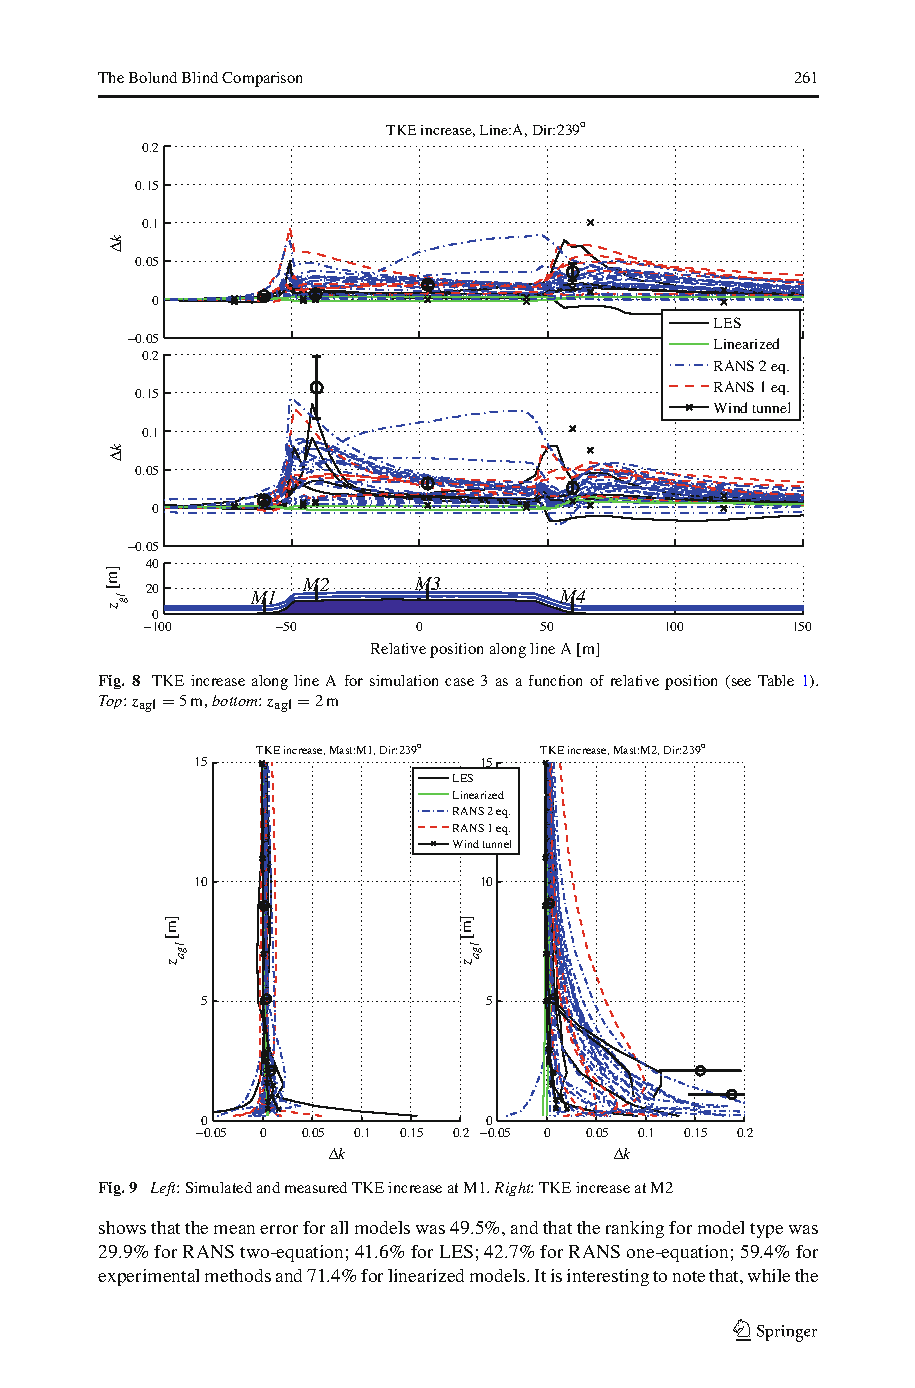
\includegraphics[width=1\linewidth,trim={2.7cm 3.8cm 1.9cm 12.5cm},clip]{bolund4.pdf}%
	
	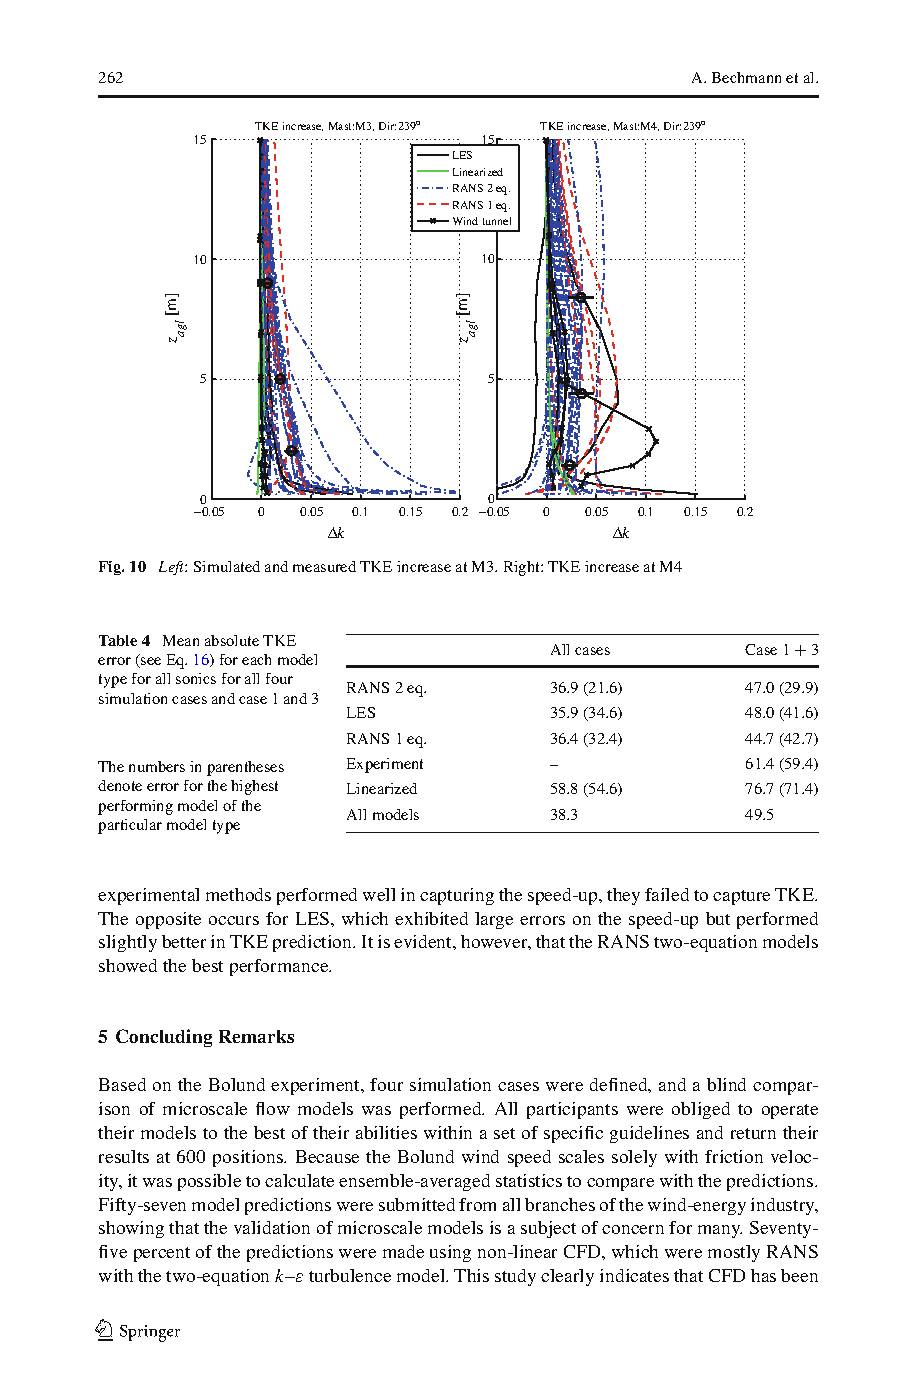
\includegraphics[width=1\linewidth,trim={2.7cm 14.3cm 1.9cm 2cm},clip]{bolund5.pdf}%
	\caption{Perfil de $\Delta k$ medido y simulado en los distintos mástiles M1-M4.}
	\label{fig:an1_delta_tke_mast}
\end{figure}
